\documentclass{beamer}
\usetheme{Luebeck}
\usecolortheme{whale}
\usepackage[]{algorithm2e}
\usepackage{amsmath}
\usepackage{graphicx}
\graphicspath{ {./imgs/} }

\setbeamertemplate{caption}[numbered]
\begin{document}
\title[Scalable EM Alignment]
{Scalable Alignment of Electron Microscope Image Sections}
\author[Zou, Ni] {Roger Zou \and Julia Ni}
\date{\today}

\frame{\titlepage}

\begin{frame}
\frametitle{Table of Contents}
\begin{itemize}
\item Overview
\item Pairwise Alignment
\item Global Stack Alignment
\item Other Attempted Methods
\item API Integration 
\item References
\item Acknowledgements 
\end{itemize}
\end{frame}

\begin{frame}
\frametitle{Overview}
\begin{itemize}
\item \textbf{Goals}
\begin{itemize}
\item Scalable alignment of 3D Electron Microscope sections of mouse brain.
\item Integration with CAJAL-3D API for easy image retrieval and upload from database.
\end{itemize}
\item \textbf{Difficulties} 
\begin{itemize}
\item Approach must be scalable.
\item $1024 \times 1024 \times 2000$ in the smallest data set $\approx 2B$ voxels.
\item Most datasets occupy TB of space; infeasible to align all at once.
\end{itemize}
\item \textbf{General Method}
\begin{enumerate}
\item Compute transformations for alignment between adjacent pairs of images using cross-correlation.
\item Globally align entire image cube using pairwise transformation parameters.
\end{enumerate}
\end{itemize}
\end{frame}

\begin{frame}
\frametitle{Pairwise Alignment}
\framesubtitle{Overview}
\textbf{Objective:} Compute transformations to align adjacent pairs of images. \\
\begin{enumerate}
\item Compute pairwise transformation parameters.
\item Improve rotation parameter through error minimization.
\item Refine transformations using image data outside pairwise images to minimize error.
\end{enumerate}
\end{frame}

\begin{frame}
\frametitle{Pairwise Alignment}
\framesubtitle{Compute Pairwise Transformation Parameters}
\textbf{Objective:} Determine transformations to align image pair. \\
For each pair of images:
\begin{enumerate}
\item Apply median filtering and histogram equalization. 
\item Take Discrete Fourier Transform, apply high-pass filter, and resample in log-polar coordinates. 
\item Find best $\rho$, $\theta$ by correlation and max picking. 
\item Rotate image, then correlate to find best translation parameters.
\item Use Support Vector Machine (SVM) to identify peak in cross-correlation of image pair. 
\item Save transformation parameters.
\end{enumerate}
\end{frame}

\begin{frame}
\frametitle{Pairwise Alignment}
\framesubtitle{Peak Identification Illustration}
\begin{figure}[p]
	\centering
	\includegraphics[width=6cm]{peak_svm.jpg}
	\caption{Motivation for Peak Identification}
	\label{fig:Peak ID}
\end{figure}
\end{frame}

\begin{frame}
\frametitle{Pairwise Alignment}
\framesubtitle{Peak Identification}
\textbf{Objective:} Determine peaks in cross-correlation of two adjacent images that correspond to translations for correct alignment. \\
\begin{itemize}
\item Support Vector Machine (SVM)
\begin{enumerate}
\item Train SVM classifier with peak features from aligned images (ground truth).
\item Partition cross-correlation of images into 9 equal parts.
\item Find point of maximum intensity in each partition.
\item Sort coordinates from greatest to least maximum intensity.
\item Classify each potential peak until a peak is found.
\item If no potential peaks are classified as peaks, then no peaks detected.
\end{enumerate}
\item Other Attempted Methods:
\begin{itemize}
\item Choose maximum values.
\item Correlate pairwise cross-correlation with normal distribution. 
\end{itemize}
\end{itemize}
\end{frame}

\begin{frame}
\frametitle{Pairwise Alignment}
\framesubtitle{Improve Rotation Parameter} 
\textbf{Objective:} Evaluate correct alignment rotation with finer level of discretization. 
\begin{enumerate}
\item Given initial estimate of rotation angle $\theta$ to align images...
\item For each $k$, iterate over small window $\theta_{new} = [\theta-k\epsilon, \theta+k\epsilon]$ in increments of $\epsilon$.
\item Compute alignment error with $\theta_{new}$ as rotation angle.
\item Update rotation parameter with angle minimizing Mean Squared Error (MSE) for image pair.
\end{enumerate}
\end{frame}

\begin{frame}
\frametitle{Pairwise Alignment}
\framesubtitle{Refine Transformation Parameters}
\textbf{Objective:} To align image pair $I_2, I_3$, use data from images $I_1$ and $I_4$. \\
\begin{enumerate}
\item Calculate pairwise transformation parameters between $I_1,I_3$ and $I_2,I_4$.
\item Obtain 2 more estimations of transformation parameters between $I_2,I_3$ using new information.
\item Determine Mean Squared Error between image pair using all estimates of transformations.
\item Pick transformation minimizing error.
\end{enumerate}
\end{frame}

\begin{frame}
\frametitle{Pairwise Alignment}
\framesubtitle{Refine Transform Parameter Illustration}
\begin{figure}[p]
	\centering
	\includegraphics[width=10cm]{tparam.jpg}
	\caption{Refine Transform Parameters}
	\label{fig:Tform Params}
\end{figure}
\end{frame}

\begin{frame}
\frametitle{Global Stack Alignment}
\textbf{Objective:} Given transformation parameters for all adjacent image pairs, compute transformation for each image in global coordinate frame.
\begin{enumerate}
\item Set global transformation parameters of previous image to that of current image. 
\item Find new rotation angle by adding previous rotation parameter to pairwise rotation angle. 
\item Find new translation parameters using previous rotation angle and pairwise translations.
\item Positive translations: shift current image. Negative translations: shift all previous images.
\item Iterate through image cube to globally align stack. 
\end{enumerate}
\end{frame}

\begin{frame}
\frametitle{Other Attempted Methods}
\begin{itemize}
\item RANSAC: Detect linear folds
\item SURF Feature Matching: Align images
\item Superpixels and Earth Mover's Distance: 'Better' error metric for image alignment
\end{itemize}
\end{frame}

\begin{frame}
\frametitle{RANSAC for Fold Detection}
\begin{itemize}
\item \textbf{Objective:} Given set of points $P$ and inlier distance $d$, outputs line of 'best' fit.
\item Procedure: 
\begin{enumerate}
\item From $P$, chooses points and finds line through them. 
\item Finds number of inliers within $d$. 
\item Based on percentage of outliers, adaptively computes number of iterations.
\item Use to split image above and below single, linear fold line.
\end{enumerate}
\item Did not encounter instances where this method is helpful, so ultimately not included in final pipeline.
\end{itemize}
\end{frame}

\begin{frame}
\frametitle{RANSAC for Fold Detection}
\framesubtitle{Results}
\begin{figure}[p]
    \centering
    \includegraphics[width=5cm]{folddetection1.jpg}
    \includegraphics[width=5cm]{folddetection2.jpg}
    \caption{Fold detection with RANSAC}
	\label{fig:RANSAC ex}
\end{figure}
\end{frame}

\begin{frame}
\frametitle{SURF Feature Detection}
\begin{itemize}
\item \textbf{Objective:} Match image features to correct rotations before cross-correlation step. 
\item Proposed method:
\begin{enumerate}
\item Use Gaussian blur on images, then resize.
\item Detect SURF (Speeded Up Robust Features) features. 
\item Match features to detect rotation angle. 
\item Rotate image, input for 2D cross-correlation.
\item Determine and save transformation parameters.
\end{enumerate}
\item Unfortunately, noise and structural similarities in EM images reduce its effectiveness.
\end{itemize}
\end{frame}

\begin{frame}
\frametitle{Superpixels and Earth Mover's Distance}
\begin{itemize}
\item \textbf{Objective:} Weigh alignment error at different regions of the image differently.
\item Mean Squared Error weighs every part of the image equally.
\item Proposed method between two images:
\begin{enumerate}
\item SLIC Superpixels to construct superpixels in both images.
\item Each superpixel center is associated with weight related to number of pixels and intensity of pixels.
\item Find the Earth Mover's Distance between the cluster centers in image pair.
\end{enumerate}
\item Unfortunately, does not appear to have any advantages compared to MSE.
\end{itemize}
\end{frame}

\begin{frame}
\frametitle{Earth Mover's Distance}
\begin{figure}[p]
	\centering
	\includegraphics[width=4cm]{emd1.png}
	\includegraphics[width=4cm]{emd2.png}
	\caption{Earth Mover's Distance}
	\label{fig:EMD}
\end{figure}
\end{frame}

\begin{frame}
\frametitle{Earth Mover's Distance}
\begin{figure}[p]
	\centering
	\includegraphics[width=7cm]{emd_eqn.jpg}
	\caption{EMD Equations}
	\label{fig:EMDEquations}
\end{figure}
\end{frame}

\begin{frame}
\frametitle{Superpixels and Earth Mover's Distance}
\framesubtitle{Results}
\begin{figure}[p]
	\centering
	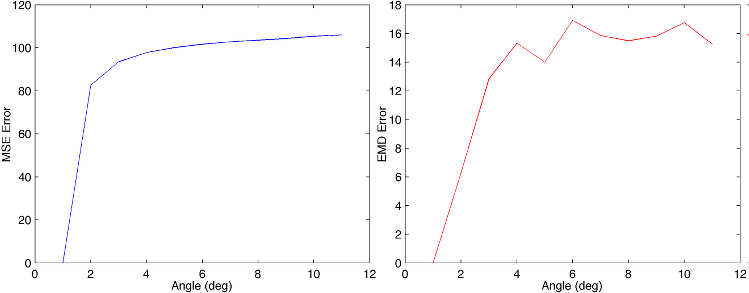
\includegraphics[width=11cm]{emderror.jpg}
	\caption{MSE vs EMD Comparison}
	\label{fig:Error Comparison}
\end{figure}
\end{frame}

\begin{frame}
\frametitle{CAJAL3D-API Integration}
\begin{itemize}
\item \textbf{Objective:} Perform affine alignment on RAMONVolume.
\item Pipeline:
\begin{enumerate}
\item Configure settings for pairwise and global alignment, and API data retrieval. 
\item Retrieve data from API. 
\item Compute transformations for pairwise alignment on sub-cubes.
\item Align cube!
\item Optional: Perform operations on aligned cube (like 3D mitochondria detection).
\item Optional: Unalign cube to original state. 
\end{enumerate}
\end{itemize}
\end{frame}

\begin{frame}
\frametitle{User Functions}
\begin{itemize}
\item \textbf{read\_api:} Retrieves data from the API and saves as RAMONVolume.
\item \textbf{alignRAMONVol:} Given a RAMONVolume, computes transformation parameters and aligns image cube.
\item \textbf{unalignRAMONVol:} Given an aligned image cube and original transformation parameters, takes inverse to revert image cube back to unaligned state.
\item \textbf{constructimgcubetransforms:} computes transformation parameters for entire data set in manageable sub-cubes.
\item \textbf{constructimgcubealignment:} Uses transformation parameters from constructimgcubetransforms, to align image cube that that data set of any specified size.
\end{itemize}
\end{frame}

\begin{frame}
\frametitle{Demo}
\textbf{DEMO!}
\end{frame}

\begin{frame}
\frametitle{References}
\begin{thebibliography}{9}
\footnotesize
\bibitem{gonzalez07}
	Rafael C. Gonzalez and Richard E. Woods,
	\emph{Digital Image Processing}.
	Prentice Hall, Third Edition, 2007
\bibitem{reddy96}
	B. Srinivasa Reddy and B. N. Chatterji,
	\emph{An FFT-Based Technique for Translation, Rotation, and Scale-Invariant Image Registration}.
	IIEEE Transactions on Image Processing Vol. 5, No. 8, 1996
\bibitem{rubner00}
	Yossi Rubner, Carlo Tomasi, Leonidas J. Guibas,
	\emph{The Earth Mover's Distance as a Metric for Image Retrieval}.
	International Journal of Computer Vision 40(2), 99-121, 2000
\bibitem{sarvaiya12}
	Jignesh N. Sarvaiya, Suprava Patnaik, Kajal Kothari,
	\emph{Image Registration Using Log Polar Transform and Phase Correlation to Recover Higher Scale}.
	Journal of Pattern Recognition Research 7(1), 90-105, 2012
\bibitem{scheffer13}
	Louis K. Scheffer, Bill Karsh, Shiv Vitaladevuni,
	\emph{Automated Alignment of Imperfect EM Images for Neural Reconstruction}.
	Report, 1-23, 2013
\bibitem{wang13}
	Peng Wang, Gang Zeng, Rui Gan, Jingdong Wang, Hongbin Zha,
	\emph{Structure-Sensitive Superpixels via Geodesic Distance}.
	International Journal of Computer Vision, 103:1-21, 2013
\end{thebibliography} 
\end{frame}

\begin{frame}
\frametitle{Acknowledgements}
Many thanks to:
\begin{itemize}
\item Chris Tralie
\item Dr. Joshua Vogelstein
\item Dr. Guillermo Sapiro
\item Will Gray 
\item Dr. Paul Bendich 
\item Dr. Robert Calderbank
\item Dr. John Harer
\item Kunal Lillaney
\item Kathy Peterson 
\item Ashleigh Thomas 
\item Duke Math RTG Group 
\end{itemize}
\end{frame}

\end{document}
